\documentclass[12pt]{article}
\usepackage{amssymb, amsmath, amsfonts, bm, graphicx, geometry}
\usepackage{tabularx, booktabs, float, enumitem, multicol, mathtools}
\usepackage{parskip} % Auto-manages paragraph spacing and removes indentations
\usepackage{siunitx} % Eases typesetting of numbers and units

\geometry{margin=1in}

\begin{document}

% --- Header Block ---
\noindent
\textbf{MA-224} \hfill \textbf{Zeshui Song} \\
\textbf{Exam 1 Corrections} \hfill \today
\vspace{2mm}
\hrule
\vspace{6mm}

% --- Body Content ---
\section*{Problem 1}
You pick a book off a bookshelf at random. Define the following events:
\begin{align*}
A &= \text{event that the book is about math}\\
B &= \text{event that the book is a textbook}\\
C &= \text{event that the cover of the book is red}
\end{align*}
\textbf{Define:}
\begin{itemize}
    \item $A = $ book is about math
    \item $B = $ book is a textbook
    \item $C = $ book has a red cover 
\end{itemize}

\begin{enumerate}[label=(\alph*), leftmargin=*]
\item Describe the event $(A \cap B')' \cup C$ in words (in class we have also used the notation $\overline{B}$ and $B^c$ for $B'$).
\paragraph{Solution}\mbox{}
\begin{itemize}
    \item $(A \cap B')$ is the event that the book is about math but not a textbook.
    \item $(A \cap B')\cup C$ is the event that the book is about math but not a textbook \textit{or the book has a red cover}
\end{itemize}
Thus, this describes the event that the book is about math and not a textbook or the book cover is red.
\item Describe the event ``the book is has a red cover and it is not a math textbook'' in symbols.
\paragraph{Solution}\mbox{}
\[C \cap (A \cap B)'\]
\item Assume 35\% of the books are about math, 55\% are textbooks, and 10\% are textbooks about math with a red cover and 7\% are textbooks about math without a red cover. What is the percentage of books which are neither about math nor a textbook?
\paragraph{Solution}\mbox{}\\
Given:\\
\begingroup
\renewcommand{\arraystretch}{1.5}
\noindent
\begin{tabular}{@{}l@{\hspace{2cm}}l@{}}
    $P(A) = 0.35$ & $P(A \cap B \cap C) = 0.10$ \\
    $P(B) = 0.55$ & $P(A \cap B \cap C') = 0.07$
\end{tabular}
\endgroup
\newpage
Find: $P(A' \cap B') = P(A\cup B)'$ (via De Morgan's laws): not about math and not a textbook.\\\\
Using the law of total probability, since $C$ and $C'$ partition the sample space, we have:
\[P(A\cap B) = P(A\cap B\cap C) + P(A\cap B\cap C')\]
\[P(A\cap B) = 0.10 + 0.07 = 0.17\]
Using the principle of inclusion-exclusion,
\begin{align*}
P(A\cup B) &= P(A) + P(B) - P(A\cap B)\\
&= 0.35 + 0.55 - 0.17\\
&= 0.73
\end{align*}
Finally, finding the complement:
\[P(A\cup B)' = 1 - P(A\cup B) = 1 - 0.73 = \boxed{0.27}\]
\paragraph{Why I lost Points}\mbox{}
I lost points because of two reasons. First, I did not understand the problem statement correctly. I thought that "nor" meant not in $A$ or not in $B$, instead of not in $A$ and not in $B$. Second, I did not see that I could use the law of total probability to find $P(A\cap B)$, being confused about how to deal with the extra intersection with $C$ and $C'$.
\end{enumerate}

\section*{Problem 2}
\begin{enumerate}[label=(\alph*), leftmargin=*]
\item Assume you randomly rearrange the letters in
\begin{center}
\textbf{OPPOSITION}\\
\end{center}
such that each arrangement of the word is equally likely. What is the probability that the rearrangement you get has identical first and second letter (for example one such arrangement is OOPSPITION, but OPPOSITION itself is not a desired arrangement)?
\paragraph{Solution}\mbox{}\\
Given 10 letters:
\begin{center}
\renewcommand{\arraystretch}{1.5}
\begin{tabular}{lc}
\toprule
\textbf{Letters} & \textbf{Count} \\
\midrule
O, O, O & 3 \\
P, P & 2 \\
I, I & 2 \\
S & 1 \\
T & 1 \\
N & 1 \\
\bottomrule
\end{tabular}
\end{center}
\underline{Number of Total Outcomes:}\\
Since switching the order of identical letters do not create a new arrangement, the order does not matter. Thus, the total number of unique arrangements is given by the multinomial coefficient:
\[\binom{10}{3,2,2,1,1,1}\]
\underline{Number of Favorable Outcomes:}
Considering cases based on which letter is repeated in the first two positions:
\begin{enumerate}
    \item[(1)] Starting with OO:\\
    The remaining letters are:
    \[O:1, P:2, I:2, S:1, T:1, N:1\]
    Using the multinomial coefficient, the number of arrangements is:
    \[\binom{8}{1,2,2,1,1,1}\]
    \item[(2)] Starting with PP:\\
    The remaining letters are:
    \[O:3, P:0, I:2, S:1, T:1, N:1\]
    Using the multinomial coefficient, the number of arrangements is:
    \[\binom{8}{3,0,2,1,1,1}\]
    \item[(3)] Starting with II:\\
    The remaining letters are:
    \[O:3, P:2, I:0, S:1, T:1, N:1\]
    Using the multinomial coefficient, the number of arrangements is:
    \[\binom{8}{3,2,0,1,1,1}\]
\end{enumerate}
Since $1!=0!=1$, we can simplify the multinomial coefficients and write the probability of the event $A$ that the arrangement has identical first and second letters as:
\[\boxed{P(A) = \frac{\binom{8}{2,2}+\binom{8}{3,2}+\binom{8}{3,2}}{\binom{10}{3,2,2}}}\]
\paragraph{Why I lost Points}\mbox{} I lost points on this problem primarily because I mixed up two counting methods for distinct and indistinguishable letters. In my original solution, I treated the first two letters as indistinguishable but treated the remaining letters as distinct. This inconsistency caused me to undercount the number of favorable outcomes. If I had consistently used the distinct-letter counting method, I should have treated the first two letters as distinct as well, accounting for the additional factor of \(2!\) corresponding to the two possible arrangements of those letters. For my revised solution, I instead treated all the letters as indistinguishable, using multinomial coefficients to count the total and favorable arrangements, staying consistent.
\item Now assume you write the letters in OPPOSITION on individual pieces of paper and throw them into a bag. You shake up the bag and randomly draw out two pieces of paper (i.e. two letters). You show them to a friend who tells you that you drew two different letters. Given this information what is the probability that you drew one consonant and one vowel?
\paragraph{Solution}\mbox{}\\
Given 10 letters: 5 vowels (O, O, O, I, I) and 5 consonants (P, P, S, T, N).\\\\
Let:
\begin{itemize}
    \item $A$ = the two letters drawn are different
    \item $B$ = the letters drawn are one consonant and one vowel
\end{itemize}
Find $P(B|A) = \frac{P(A\cap B)}{P(A)}$.\\\\
\underline{Find $P(A)$}:\\
There are $\binom{10}{2}$ ways to draw two letters from the bag.\\\\
However, this count \textit{includes the cases where the two letters drawn are the same}. Since we know that the two letters drawn are different, we need to subtract the cases where the two letters drawn are the same.\\\\
There are 3 O's, 2 P's, and 2 I's:
\[\binom{3}{2} + \binom{2}{2} + \binom{2}{2}\]
Therefore:
\[P(A) = \frac{\binom{10}{2}-\binom{3}{2}-\binom{2}{2}-\binom{2}{2}}{\binom{10}{2}}\]
\underline{Find $P(A\cap B)$}\\
Noting that every vowel-cosonant pair is already a favorable outcome since they are different letters, we can find $P(A\cap B)$ by counting the number of ways to draw one vowel and one consonant.\\\\
By multiplication principle, there are
\[\underbrace{5}_{\text{ways to select one vowel}}\cdot \underbrace{5}_{\text{ways to select one consonant}} = 25\]
Therefore:
\[P(A\cap B) = \frac{25}{\binom{10}{2}}\]
Finally, we can find $P(B|A)$:
\[\boxed{P(B|A)=\frac{25}{\binom{10}{2}-\binom{3}{2}-\binom{2}{2}-\binom{2}{2}}}\]
\end{enumerate}
\paragraph{Why I lost Points}\mbox{} In my original solution, I did not consider the fact that I would need to compute the \textit{conditional probability}, and instead only computed for the probability of drawing one consonant and one vowel. By including the condition that the two letters drawn are different in the corrected solution, the probability is now narrowed down to a smaller sample space.
\section*{Problem 3}
There are four raffle prizes (A, B, C, and D) available, and I have enough money to buy exactly one raffle ticket. If I buy a ticket for prize A I have a 60\% chance of getting it. If I buy a ticket for prize B I have a 45\% chance of getting it. If I buy a ticket for prize C I have a 20\% chance of getting it. If I buy a ticket for prize D I have a 15\% chance of getting it. I roll a fair four sided die to decide which raffle to enter.\\\\
\textbf{Define Events and Givens:}\\
Let $W$ = winning.
\[
P(A)=P(B)=P(C)=P(D)=0.25
\]
\begin{center}
\renewcommand{\arraystretch}{1.5}
\begin{tabular}{ll}
$A=\{\text{win raffle for A}\}$ & $P(W\mid A)=0.6$ \\
$B=\{\text{win raffle for B}\}$ & $P(W\mid B)=0.45$ \\
$C=\{\text{win raffle for C}\}$ & $P(W\mid C)=0.2$ \\
$D=\{\text{win raffle for D}\}$ & $P(W\mid D)=0.15$
\end{tabular}
\end{center}
\begin{enumerate}[label=(\alph*), leftmargin=*]
\item What is the probability I win a prize?
\paragraph{Solution}\mbox{} Find $P(W)$ using the law of total probability:
\[
P(W)=P(A)P(W\mid A)+P(B)P(W\mid B)+P(C)P(W\mid C)+P(D)P(W\mid D)
\]
\[
\boxed{P(W)=0.25(0.6+0.45+0.2+0.15)}
\]
\newpage
\item Assume I did get a prize what is the probability I entered the raffle for Prize C?
\paragraph{Solution}\mbox{} Find $P(C\mid W)$ using Bayes' theorem:
\[
P(C\mid W)=\frac{P(C\cap W)}{P(W)}
=\frac{P(W\cap C)}{P(W)}
=\frac{P(W\mid C)P(C)}{P(W)}
\]
\[
\boxed{
=\frac{(0.2)(0.25)}{(0.25)(0.6+0.45+0.2+0.15)}
}
\]
\item Now assume your friend buys one ticket for each raffle, and whether or not they win each raffle is mutually independent of the others. With these assumptions what is the probability your friend wins at least one prize?
\paragraph{Solution}\mbox{}\\
Let
\begin{center}
\renewcommand{\arraystretch}{1.5}
\begin{tabular}{ll}
$A=\{\text{win A}\}$ & $B=\{\text{win B}\}$ \\
$C=\{\text{win C}\}$ & $D=\{\text{win D}\}$
\end{tabular}
\end{center}
\[
P(\text{win at least 1 prize})=1-P(\text{win no prizes})
\]
\[
P(\text{win no prize})=P(A'\cap B'\cap C'\cap D')
\]
By mutual independence of the events $A, B, C, D$:
\[
=P(A')P(B')P(C')P(D')
\]
\[
=[1-P(A)][1-P(B)][1-P(C)][1-P(D)]
\]
\[
\boxed{
P(\text{win at least 1 prize})
=1-(1-0.6)(1-0.45)(1-0.2)(1-0.15)
}
\]
\end{enumerate}

\section*{Problem 4}
Assume you have one unbiased five-sided die (with sides labeled 1, 2, 3, 4, 5) and one unbiased four-sided die (with sides labeled 1, 2, 3, 4). Assume you roll each die (the rolls are independent of each other). Let the random variable $X$ denote the outcome of the five-sided die and let $Y$ denote the outcome of the four-sided die. Let $Z = |3Y - 2X|$.\\\\
\textbf{Given:}
\[X = {1,2,3,4,5}\]
\[Y = {1,2,3,4}\]
\[Z = |3Y - 2X|\]
\newpage
\begin{enumerate}[label=(\alph*), leftmargin=*]
\item Write the p.m.f of $Z$.
\paragraph{Solution}\mbox{}\\
\underline{Total Number of Possible Outcomes:}\\
There are 5 possible outcomes of the 5-sided die and 4 possible outcomes of the 4-sided die. Thus, there are $5\cdot 4 = 20$ total possible outcomes.\\\\
\underline{Number of Favorable Outcomes:}\\
I can find the number of favorable outcomes more efficiently by organizing the outcome in a table of $X$ and $Y$ values, and then computing the corresponding $Z$ value for each pair $(X,Y)$.
\[
Z = |3Y - 2X|
\]
\begin{center}
\begin{tabular}{c|ccccc}
\hline
$Y / X$ & 1 & 2 & 3 & 4 & 5 \\
\hline
1 & 1  & 1 & 3 & 5 & 7 \\
2 & 4  & 2 & 0 & 2 & 4 \\
3 & 7  & 5 & 3 & 1 & 1 \\
4 & 10 & 8 & 6 & 4 & 2 \\
\hline
\end{tabular}
\end{center}
Thus, the p.m.f. of $Z$ is:
\begin{center}
\begin{tabular}{c|cc}
\hline
$z$ & Count & $P(Z=z)$ \\
\hline
0  & 1 & $1/20$ \\
1  & 4 & $4/20$ \\
2  & 3 & $3/20$ \\
3  & 2 & $2/20$ \\
4  & 3 & $3/20$ \\
5  & 2 & $2/20$ \\
6  & 1 & $1/20$ \\
7  & 2 & $2/20$ \\
8  & 1 & $1/20$ \\
10 & 1 & $1/20$ \\
\hline
\end{tabular}
\end{center}
\paragraph{Why I lost Points}\mbox{} I lost points mostly because I didn't think to organize the outcomes in a table. For my original solution, I was brute forcing the calculations for each possible combination of $X$ and $Y$ to match the corresponding $Z$ value, which was inefficient and prone to error. So I lost points on missing out on some of the counts for the p.m.f. of $Z$.
\newpage
\item Draw a probability histogram for $Z$.
\paragraph{Solution}\mbox{}
\begin{center}
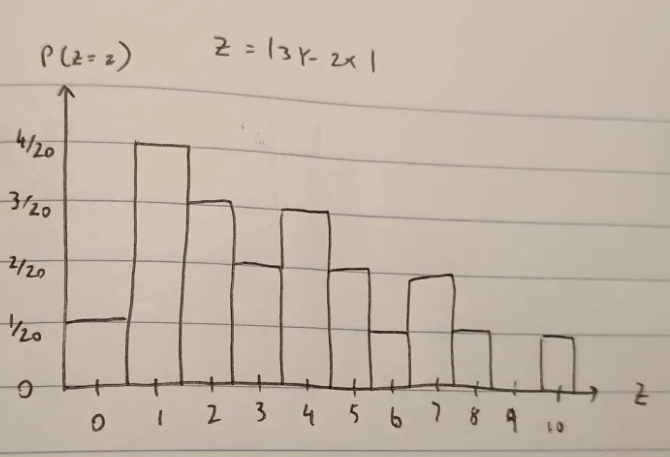
\includegraphics[width=0.8\textwidth]{histogram.png}
\end{center}
\paragraph{Why I lost Points}\mbox{} I lost points mostly because I was running out of time after the previous part of the problem and so I made mistake sin the vertical axis labels and the probabilities were wrong because the previously computed p.m.f. of $Z$ was incorrect. I also didn't label the horizontal axis, denoting the values of $Z$.
\item Let $A$ be the event that $Z=1$. Let $B$ be the event that the five-sided die landed on a 2. Are the events $A$ and $B$ independent? Justify your answer.
\paragraph{Solution}\mbox{}\\
Given:
\begin{itemize}
    \item $P(A) = 4/20$
    \item $P(B) = 1/5$
\end{itemize}
For $X=2$, the possible values of $Y$ are 1, 2, 3, 4. Thus, the possible values of $Z$ are:
\[Z={1,2,5,8}\]
Thus, there is only one possible outcome where $Z=1$ and $X=2$,
\[\implies P(A \cap B) = \frac{1}{20}\]
Testing for the independence of $A$ and $B$:
\[P(A \cap B) = P(A) \cdot P(B)\]
\[\frac{1}{20} = (\frac{4}{20}) \cdot (\frac{1}{5})\]
\[\frac{1}{20} \neq \frac{1}{25}\]
So the events $A$ and $B$ are not independent.
\paragraph{Why I lost Points}\mbox{} I lost points because I miscounted the number of favorable outcomes for $P(A\cap B)$ in my original solution. Otherwise, I had the correct approach to test for independence of the two events.
\end{enumerate}

\section*{Problem 5}
Prove or disprove the following statements. Assume all events occur with non-zero probability.

\begin{enumerate}[label=(\alph*), leftmargin=*]
\item If $\mathbb{P}(A\mid B)>\mathbb{P}(A)$ then $\mathbb{P}(B\mid A)>\mathbb{P}(B)$.
\paragraph{Solution}\mbox{}\\
Given:
\[
P(A\mid B)>P(A)
\]
By the definition of conditional probability:
\[
\frac{P(A\cap B)}{P(B)}>P(A)
\]
Multiplying both sides by $P(B)$:
\[
P(A\cap B)>P(A)P(B)
\]
Since $P(A\cap B)=P(B\cap A)$:
\[
\frac{P(B\cap A)}{P(A)}>P(B)
\]
Therefore:
\[
\boxed{P(B\mid A)>P(B)}
\]

\item If $\mathbb{P}(A)>\mathbb{P}(B)$ then $\mathbb{P}(A\mid C)>\mathbb{P}(B\mid C)$.
\paragraph{Solution}\mbox{}\\
Given: $P(A)>P(B)$\\\\
Assuming that $P(A\mid C)>P(B\mid C)$, by the definition of conditional probability:
\[
\frac{P(A\cap C)}{P(C)}>\frac{P(B\cap C)}{P(C)}
\]
Since $P(C)$ is non-zero, we can multiply both sides by $P(C)$:
\[
P(A\cap C)>P(B\cap C)
\]
Since we only know that $P(A)>P(B)$, we cannot conclude that $P(A\cap C)>P(B\cap C)$.\\\\
This statement can be disproven by a counterexample where $P(A)>P(B)$ but $P(A\cap C)<P(B\cap C)$.\\\\
Suppose:
\[
A\cap C=\varnothing,\qquad B\subseteq C,\qquad P(A)>P(B)>0
\]
Such that:
\[P(A\cap C)=0,\qquad P(B\cap C)=P(B)\]
Since $P(B)>0$, the statement $P(A\cap C)>P(B\cap C)$ is false, and thus the statement $P(A\mid C)>P(B\mid C)$ is also false.
\end{enumerate}

\end{document}
